\subsubsection{Downstream Task Fine-tuning: Portrait Image-to-Video Generation}
We perform supervised finetuning of our I2V model on two million portrait videos to enhance human's motion and overall aesthetics. In addition to the standard data filtering pipeline described in section \ref{sec:data}, we also apply face and body detectors to filter out the training videos which have more than five persons. We also remove the videos in which the main subjects are small. Finally, the rest videos will be manually inspected to obtain the final high-quality portrait training dataset.

Regarding training, we adopt a progressive fine-tuning strategy, gradually unfreezing the model parameters of the respective layers while keeping the rest frozen during finetuning. This approach allows the model to achieves high performance in the portrait domain without compromising much of its inherent generalization ability, guaranteeing commendable performance in natural landscapes, animals, and plants domains. Moreover, our model also supports video interpolation by using the first and last frames as conditions. We randomly drop the text conditions at certain probability during training to enhance the model's performance. Some demo results are shown in Fig. \ref{fig:portrait_i2v}.

\begin{figure}[h]
    \centering
    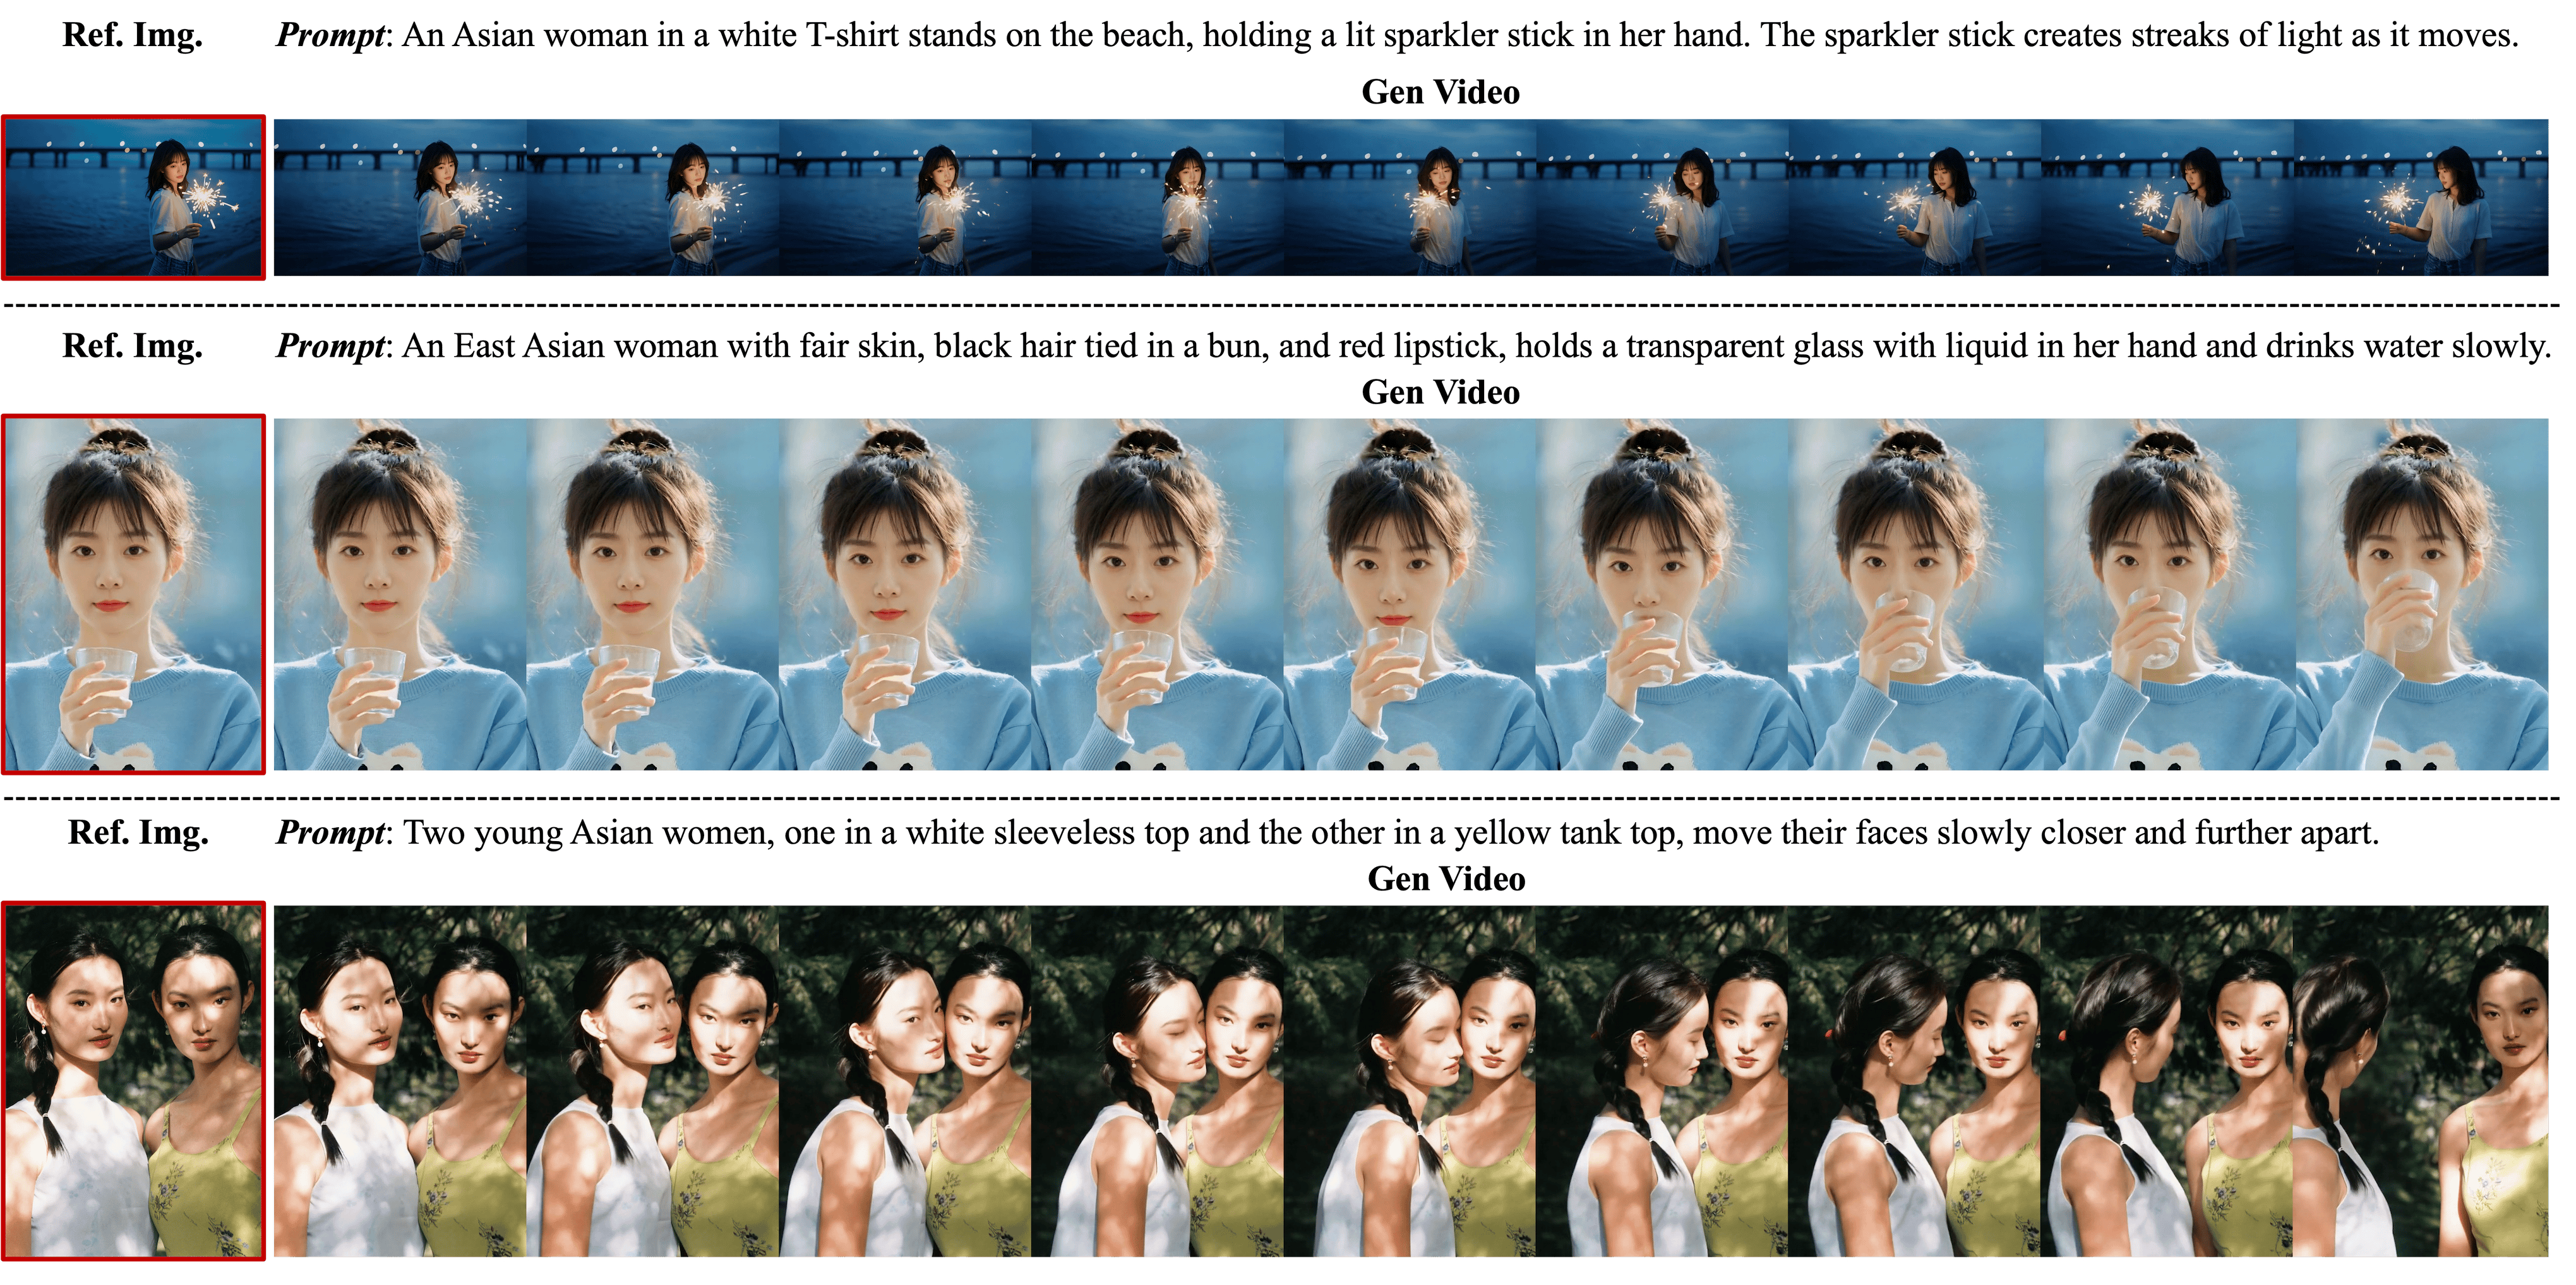
\includegraphics[width=\linewidth]{applications//app_figures/portrait_to_video_new.png}
    \caption{Sample results of our portrait I2V model.}
    \label{fig:portrait_i2v}
\end{figure}